\subsection{Background}

\frame{
	\frametitle{Background}
	\begin{columns}
		\begin{column}{0.15\textwidth}
			\begin{center}
				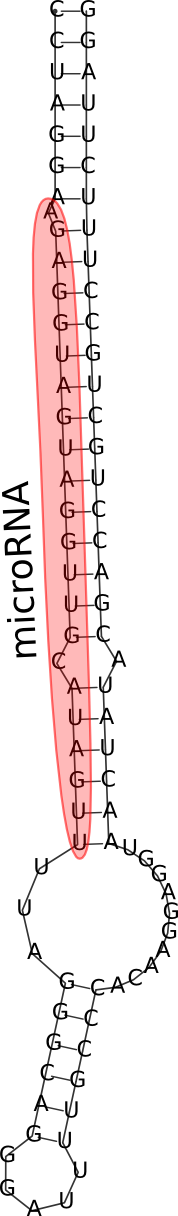
\includegraphics[width=0.6\textwidth]{res/premirna.png}
			\end{center}
		\end{column}

		\begin{column}{0.9\textwidth}
			\begin{itemize}
				\item MicroRNAs (miRNAs) play an essential role in post-transcriptional gene regulation. \pause
					\vspace{10pt}
				\item Precursors of miRNA (pre-miRNAs) are characterized by hairpins structure. \pause
					\vspace{10pt}
				\item A large amount of similar sequences can be folded into this kind of structure. \pause
					\vspace{10pt}
				\item Machine learning algorithms have been proposed to predict which sequences are likely to contain a miRNA.
			\end{itemize}
		\end{column}
	\end{columns}
}

\frame{
	\frametitle{But, there are some problems with ML methods}
	\begin{columns}
		\begin{column}{0.15\textwidth}
			\begin{center}
				
\includegraphics[width=\textwidth]{res/lupa.png}
			\end{center}
		\end{column}

		\begin{column}{0.9\textwidth}
			\begin{itemize}
				\item Datasets used are not representative of the wide variety of negative examples. \\
					$\rightarrow$ Use all hairpins of the genome for validation.
					\pause \vspace{10pt}
				\item The performance measures used underestimate the effect of imbalance. \\
					$\rightarrow$ Take into account the number of false positives.
					\pause \vspace{10pt}
				\item The validation methodology does not imitate a real prediction task. \\
					$\rightarrow$ Test on sequences from unseen species.
					\pause
			\end{itemize}
			\vspace{10pt}
			\centering
			\emph{Taking into account these points, simple sequence alignment works better than machine learning methods.}
		\end{column}
	\end{columns}
}

\subsection{Motivation}
\frame{\frametitle{Can it be done better?}
	\includegraphics<1>[width=\textwidth]{res/better1.pdf}%
	\includegraphics<2>[width=\textwidth]{res/better2.pdf}%
	\includegraphics<3>[width=\textwidth]{res/better3.pdf}%
	\includegraphics<4>[width=\textwidth]{res/better4.pdf}
}
